\graphicspath{{../results/figures/theory/}{../results/figures/}}
\chapterepigraph{Men do not know how what is at variance agrees with itself. It
is an attunement of opposite tensions, like that of the bow and the lyre.}{Heraclitus}
{\textit{Fragments}}

\begingroup
\let\clearpage\relax
\let\cleardoublepage\relax
\chapter{The many-body problem}
\label{sec:theory}
\endgroup

The system is $N$ electrons in a two-dimensional harmonic trap, repelling one another
through the Coulomb interaction. Its Hamiltonian is elementary, and three of its properties
make the numerical solution difficult.

The electrons are identical fermions, so the wavefunction changes sign under exchange, and
that sign structure is the expensive part of the problem. The interaction diverges where
two electrons meet, so the local energy $\hat H\Psi/\Psi$ diverges with it unless the
wavefunction is constructed to cancel the divergence. And the kinetic term is a second
derivative, which exposes any method that evaluates the energy pointwise to the curvature
of the function it is given.

\section{The many-body problem}
\label{sec:qm-setup}

A quantum state is a normalised vector in a complex Hilbert space, and in the coordinate
representation $\psi(x)=\braket{x|\psi}$ is the wavefunction. Which basis one expands in is
not a formality: choosing it to match the physics (harmonic-oscillator orbitals for confined charges, plane waves for periodic systems) is what makes a representation compact, and it is
why the orbitals of Chapter~\ref{ch:trial_wavefunction} are those of the trap itself.

For $N$ particles the space is the $N$-fold tensor product $\mathcal H_1^{\otimes N}$, and a
fermionic state expands exactly in Slater determinants built from $N$ distinct spin-orbitals,
$\ket\Psi=\sum_I C_I\ket{\Phi_I}$. That expansion is exact and, as \S\ref{sec:fci} makes
precise, unaffordable.

We work in atomic units ($\hbar=m_e=e=1$) with the many-body Hamiltonian
\begin{equation}
H = -\frac12 \sum_{i=1}^N \nabla_{\mathbf r_i}^2
    \;+\; \sum_{i=1}^N V_{\mathrm{ext}}(\mathbf r_i)
    \;+\; \sum_{i<j} V_{\mathrm{int}}(|\mathbf r_i-\mathbf r_j|),
\qquad H\Psi(R)=E\Psi(R),
\label{eq:manybody-H}
\end{equation}
where $R=(\mathbf r_1,\ldots,\mathbf r_N)$ and $\Psi$ is normalised. Identical particles
restrict $\Psi$ to a symmetry sector, antisymmetric for the fermions studied here. For these
quantum dots $V_{\mathrm{ext}}(\mathbf r)=\tfrac12\omega^2r^2$ and $V_{\mathrm{int}}(r)=1/r$
in two dimensions. Everything that follows approximates the lowest eigenpair of
Eq.~\eqref{eq:manybody-H}.

\section{Correlation, closed shells, and the cost of exactness}
\label{sec:secondquant}
\label{sec:fci}

Three ideas from electronic structure are used throughout this thesis and computed nowhere in
it. They are what the accuracy claims of later chapters are calibrated against.

The first is \emph{correlation energy}. Hartree--Fock approximates the ground state by a
single determinant whose orbitals are themselves optimised, each electron moving in the mean
field of the others; the correlation energy $\Delta E=E_{\rm exact}-E_{\rm HF}$ is whatever
that cannot reach. It is a small fraction of the total and essentially all of the difficulty,
which is why a method can look converged in total energy while representing the correlation
badly---a distinction Chapter~\ref{ch:kernel} makes quantitative.

The second is \emph{closed-shell structure}. When the occupied orbitals fill complete shells
the determinant is a spin singlet and is unique, with no degenerate manifold to choose from.
Those particle numbers, $N\in\{2,6,12,20\}$ in a two-dimensional parabolic trap, are the ones
studied here.

The third is \emph{exactness within a basis}, and its price. Expanding in all $N$-electron
determinants of a given one-particle basis and diagonalising gives the exact ground state
within that basis; what cannot be avoided is the $\binom{M}{N}$ growth of the space itself,
which for the twenty-electron dot puts the determinant count far beyond reach. That
combinatorial wall is what motivates variational methods. The occupation-number formalism of
second quantisation, in which antisymmetry is carried by anticommuting creation and
annihilation operators, not by the wavefunction, is the usual language for all three;
our own ansatz is first-quantised throughout, so it appears here as vocabulary rather than
machinery.

Our determinant is built from harmonic-oscillator orbitals, not self-consistent
Hartree--Fock ones, and our external benchmark is diffusion Monte
Carlo~\cite{Pederiva2000-QD-DMC}, which for these systems is both more accurate than an
affordable configuration-interaction calculation and available at the particle numbers we
care about.

\section{Quantum dots}
\label{sec:quantumdots}

\subsection{Model and units}
We consider $N$ spin-$\tfrac12$ fermions in $d{=}2$ with harmonic confinement and Coulomb repulsion,
\[
H \;=\; \sum_{i=1}^N\!\bigg(-\tfrac12\nabla_{\mathbf r_i}^2 + \tfrac12 \omega^2 r_i^2\bigg)
\;+\;\sum_{i<j}\frac{1}{|\mathbf r_i-\mathbf r_j|}, \qquad (\hbar=m_e=e=1).
\]
Spin does not appear in $H$, so the eigenstates can be classified by $S$ and $S_z$ and the
spatial problem solved at fixed spin assignment. For more than two identical fermions a
spin-adapted eigenstate of $S^2$ is in general a sum of spatial--spin products, not a single one; what we use computationally is the weaker and sufficient statement that with the
numbers of up- and down-spin electrons held fixed, the antisymmetriser factorises and the
spatial problem may be treated on its own.

\subsection{One–particle structure and shell filling}
We use two-dimensional harmonic-oscillator spin–orbitals. In the implementation these are
the \emph{Cartesian} 2D-HO eigenstates $\{\phi_{n_x n_y}(\mathbf r)\chi_\sigma\}$ with
energies $E_{n_x n_y}=\omega (n_x+n_y+1)$ and spin $\sigma\in\{\uparrow,\downarrow\}$.
The principal index $k=n_x+n_y$ labels a shell of $(k{+}1)$ degenerate spatial states, each
twofold spin-degenerate; for the closed shells studied here this Cartesian basis spans the
same filled subspace as any complete basis of those shells, so the reference determinant is
basis-independent. Filling from the bottom yields the \emph{closed-shell} electron numbers
\[
N_{\mathrm{closed}}=(K{+}1)(K{+}2), \quad K=0,1,2,\dots \quad (2,6,12,20,30,\dots).
\]
All other $N$ correspond to a \emph{partially filled} top shell (open shell), with a degenerate
noninteracting manifold.

\subsection{Spin structure and Slater form}
Write single-particle spin-orbitals as $\varepsilon_\alpha(x)=\phi_\alpha(\mathbf r)\,\chi_{\sigma}(s)$,
with $x=(\mathbf r,s)$. Because $\chi_\uparrow$ and $\chi_\downarrow$ are orthogonal and $H$ is
spin-independent, the Slater determinant simplifies:

\paragraph{Closed shells.}
For even $N$ with doubly occupied spatial orbitals
$\{\phi_1,\ldots,\phi_{N/2}\}$, the determinant factorizes into two identical spatial determinants,
one for each spin:
\[
\Psi_{\mathrm{closed}}(X)
=\frac{1}{(N/2)!}\;
\det[\phi_a(\mathbf r_i)]_{i\in\uparrow,a=1..N/2}\;
\det[\phi_a(\mathbf r_j)]_{j\in\downarrow,a=1..N/2}\;\times\; \Xi_{S=0,S_z=0},
\]
where $\Xi$ is the singlet spin function. In the computational representation this last
factor is not carried: fixing which electrons are spin-up and which spin-down makes the full
spin-orbital determinant block diagonal, and the product of the two spatial determinants
\emph{is} the ansatz. This has the \emph{form} of a restricted closed-shell determinant, but
its orbitals are the
harmonic-oscillator eigenstates of the trap, not orbitals optimised self-consistently in
the mean field of the other electrons. It is therefore the closed-shell
\emph{non-interacting} reference, not an RHF one, and no self-consistent-field calculation
is performed anywhere in this thesis. The distinction matters for how the later results
should be read: everything the correlator and the backflow achieve is measured against a
determinant that has not been given the benefit of a mean field, so what they recover
includes the orbital relaxation an HF calculation would have supplied as well as the
correlation beyond it.

% \paragraph{Open shells.}
% When the top shell is partially filled, the noninteracting ground space is degenerate.
% Physically relevant sectors are labeled by $(N,S,S_z,L_z)$. One may:
% (i) use ROHF (doubly occupied core $+$ singly occupied open-shell orbitals, spin-adapted to
% a chosen $(S,S_z)$), (ii) allow UHF (different spatial orbitals for $\uparrow,\downarrow$), or
% (iii) build a small multi-determinant reference within the top shell to enforce good $S$ and $L_z$.
% In our variational approach we keep a compact Slater reference (RHF for closed shells; ROHF/UHF
% or a minimal multi-determinant for open shells) and capture residual correlation with a Jastrow/PINN
% correlation factor.

\subsection{Kato cusp conditions in two dimensions}
\label{subsec:cusp}

For Coulomb interactions the potential diverges as $1/r$ at coalescence. Finiteness of the
local energy
\[
E_L(R)=\frac{(H\Psi)(R)}{\Psi(R)}
\]
requires that the kinetic singularity cancels the $1/r$ divergence. Kato’s theorem, first proved in \cite{Kato1957-EigenfunctionsManyParticle}, gives the
necessary short–distance behaviour of the (spherically averaged) wavefunction. Let $r_{ij}$ be the
interparticle distance, $\mu_{ij}=m_i m_j/(m_i+m_j)$ the reduced mass (in a.u.), $Z_i$ the charge
number (electron $Z=-1$, nucleus $Z=+Z_A$), and $D$ the spatial dimension. Then
\[
\left.\frac{\partial}{\partial r_{ij}}\ln \overline{\Psi}\right|_{r_{ij}\to 0}
\;=\; \frac{2\,\mu_{ij}\,Z_i Z_j}{D-1}
\quad\text{(s-wave / opposite-spin channel)}.
\]
For \emph{identical fermions} the s-wave is excluded; the leading channel is $p$-wave
(relative angular momentum $k=1$), and the wavefunction carries a linear node at
coalescence. The cusp condition then applies to the \emph{regular part} left after that node
is factored out, and this distinction is easy to lose. Writing
$\overline\Psi(r)=r\,\overline{u}(r)$ with $\overline u$ regular and nonzero at contact, the
logarithmic derivative of the full wavefunction diverges,
$\partial_r\ln\overline\Psi = 1/r + \partial_r\ln\overline u$, so it is $\overline u$ and not
$\overline\Psi$ that obeys a finite cusp condition:
\[
\left.\frac{\partial}{\partial r_{ij}}\ln \overline{u}\right|_{r_{ij}\to 0}
\;=\; \frac{2\,\mu_{ij}\,Z_i Z_j}{2k + D - 1}
\;=\; \frac{2\,\mu_{ij}\,Z_i Z_j}{D+1}
\quad\text{(like-spin, $k=1$)}.
\]
In a Slater--Jastrow form the antisymmetric factor supplies the linear zero and the Jastrow
supplies $\overline u$, so this is exactly a condition on the Jastrow slope---which is how it
is imposed in Chapter~\ref{ch:trial_wavefunction}.

\paragraph{Specializing to 2D electrons (atomic units).}
With $m_e=1$ and $\mu_{ee}=1/2$:
\[
\boxed{\ a_{ee}^{\uparrow\downarrow}=\left.\frac{\partial}{\partial r_{ij}}\ln \overline{\Psi}\right|_{0}=1\ ,\qquad
a_{ee}^{\uparrow\uparrow}=\left.\frac{\partial}{\partial r_{ij}}\ln \overline{u}\right|_{0}=\tfrac13\ .\ }
\]
The two derivatives are taken on different objects: the full spherically averaged
wavefunction in the antiparallel case, where it is finite at contact, and its regular part in
the parallel case, where the antisymmetric node has been removed.
The like-spin value follows from the $p$-wave (linear-node) analysis carried out in full
in Appendix~\ref{app:coulomb:cusp}, the canonical derivation used throughout this thesis;
it gives the familiar $\tfrac14$ in three dimensions and $\tfrac13$ here in two. The 2D
like-spin cusp is therefore \emph{not} simply half the opposite-spin value---a
coincidence that holds only in 3D---and the implemented value is $1/(D+1)=\tfrac13$.
For electron–nucleus coalescence ($\mu_{eA}\!\approx\!1$, $Z_i Z_j=-Z_A$):
\[
\boxed{\ a_{eA}=\left.\frac{\partial}{\partial r_{iA}}\ln \overline{\Psi}\right|_{0}=-2 Z_A\ .\ }
\]

\paragraph{Why this matters.}
These conditions ensure the kinetic energy’s $r^{-1}$ singularity cancels the Coulomb $r^{-1}$
term so that $E_L$ remains finite as particles coalesce. Enforcing the cusp explicitly improves conditioning.

\section{Structural diagnostics and Wigner markers}
\label{sec:wigner-markers-theory}

A Wigner molecule is not defined by a single number, so the crossover has to be read from
several markers at once. This section says what each one measures and why it responds to
Wigner order; the estimators, thresholds and stability protocol are defined once, in the
Analysis chapter (\S\ref{sec:analysis-struct}), and the measurements themselves are in
Chapter~\ref{ch:results}.

\paragraph{Radial localisation.} The pair distribution $g(r)$ and the radial probability
$P(r)$ say how far apart the electrons sit and how tightly that distance is fixed. The informative quantity is not the typical radius, which simply grows as the trap weakens, but
the \emph{ratio} of the radial width to it. A distribution that becomes relatively narrower
around a growing radius is a shell stiffening; one that merely dilates is a droplet
expanding. This is the finite-system analogue of a Lindemann criterion.

\paragraph{Shell topology.} In a parabolic trap the classical minimum energy configuration
is a set of concentric rings with definite occupancies---$(1,5)$ at $N{=}6$, $(3,9)$ at
$N{=}12$~\cite{schweigert1994spectralpropertieschargedparticles,Kong_2002}. Detecting those
occupancies frame by frame turns a qualitative picture into a distribution over topologies,
which is what makes it possible to say that a state is \emph{mostly} $(3,9)$ with real
weight on $(2,10)$---a rotating molecule fluctuating between near-degenerate shellings
rather than a single frozen crystal.

\paragraph{Orientational order.} Radial structure alone cannot distinguish a ring of
electrons at fixed angular spacing from a ring free to slide. The bond-orientational order
parameter $\Phi_m$ measures $m$-fold angular order on a detected ring after removing global
rotation, and an angular Lindemann number measures how stiff those spacings are. Both are
standard in two-dimensional Coulomb and Yukawa
systems~\cite{Mazars_2008,Filinov_2001}, and together with the radial markers they separate
angular from radial melting---the two need not happen at the same $\omega$.

\paragraph{Classical scaling.} Finally, the strong-coupling limit makes a parameter-free
prediction: inter-particle distances should approach $r\propto\omega^{-2/3}$. Fitting the
measured exponent and watching it approach $-2/3$ from above is an external check on the
whole picture, since nothing in the ansatz knows about that number.

\paragraph{How to read them together.} As $\omega$ falls, the width ratios and angular
Lindemann numbers shrink, shell gaps sharpen, the shell-resolved $|\Phi_m|$ rise above their
finite-ring random-angle baseline, and the radial exponent approaches its classical value. No one of
these is decisive---a narrow $P(r)$ can be an artefact of poor sampling, and a large
$|\Phi_m|$ can be a fluctuation on a short chain---but they fail in different ways, which is
why Chapter~\ref{ch:results} reports them together and Chapter~\ref{ch:analysis} states the
stability checks each one is subjected to. Quantum Wigner markers in parabolic dots are
reviewed in Refs.~\cite{Egger_1999,manninen2007metalclustersquantumdots,Filinov_2001,Mazars_2008}.

%%%%%%%%%%%%%%%%%%%%%%%%%%%%%%%%%%%%%%%%%%%%%%%%%%%%%%%%%%%%%%%%%%%%%
\section{Quantum Monte Carlo benchmarks}
\label{sec:qmc-theory}

Two stochastic methods supply the numbers this thesis is measured against, and the
difference between what they guarantee is the whole of its external evidence. Variational
Monte Carlo optimises a trial state under the variational principle. Diffusion Monte Carlo
projects toward the ground state in imaginary time. Only the first is what we do; only the
second is what we are scored against; and neither is exact for fermions.

\subsection{Variational Monte Carlo}
\label{subsec:vmc-theory}

For any normalised trial state $\Psi_T(\mathbf R;\boldsymbol\alpha)$ the Rayleigh quotient
\[
E[\Psi_T] = \frac{\braket{\Psi_T|\hat H|\Psi_T}}{\braket{\Psi_T|\Psi_T}} \;\ge\; E_0
\]
bounds the exact ground-state energy from above, so minimising it over $\boldsymbol\alpha$
can only improve the estimate. Writing the expectation as an average of the \emph{local
energy}
\begin{equation}
  E_L(\mathbf R) \;=\; \frac{\hat H\Psi_T(\mathbf R)}{\Psi_T(\mathbf R)}
  \label{eq:local-energy-theory}
\end{equation}
over configurations drawn from $P(\mathbf R)=|\Psi_T(\mathbf R)|^2/\!\int|\Psi_T|^2$ turns
the integral into a sampling problem,
\[
  E[\Psi_T] \;\approx\; \frac{1}{N_{\rm MC}}\sum_{i} E_L(\mathbf R_i),
\]
with the configurations generated by Metropolis--Hastings~\cite{Metropolis1953} at
acceptance
\[
A(\mathbf R \to \mathbf R') = \min\!\left(1,\;
\frac{|\Psi_T(\mathbf R')|^2}{|\Psi_T(\mathbf R)|^2}\,
\frac{T(\mathbf R'\to\mathbf R)}{T(\mathbf R\to\mathbf R')}\right),
\]
optionally drifted by the quantum force $\mathbf F=2\nabla\ln|\Psi_T|$ toward regions of
high density~\cite{KalosLevesqueVerlet1974-ImportanceSampling}.

\paragraph{The zero-variance principle.}
One property of Eq.~\eqref{eq:local-energy-theory} does more work in this thesis than the
energy itself. If $\Psi_T$ were an exact eigenstate, $\hat H\Psi_T=E\Psi_T$ pointwise, and
$E_L$ would be \emph{constant} over the whole of configuration space. Its variance
\begin{equation}
  \Var(E_L) \;=\; \big\langle E_L^2\big\rangle - \big\langle E_L\big\rangle^2
  \label{eq:varEL-theory}
\end{equation}
therefore vanishes only at an exact eigenstate, and decreases as the trial state improves.
This makes it a measure of wavefunction quality that is independent of any external
reference---which matters here for two reasons. It keeps saying something after the energy
has saturated, when two ansätze agree to four figures and the energy can no longer tell
them apart. And it is defined on the state rather than on any component of it, so it
survives changes of parameterisation that quantities such as a component's rank do not.
Chapter~\ref{ch:kernel} uses it in both roles.

\subsection{Diffusion Monte Carlo, and the fixed-node constraint}
\label{subsec:dmc-theory}

DMC removes the dependence on a trial state by projection. In imaginary time
$\tau=it$ the Schr\"odinger equation becomes a diffusion equation,
\[
-\frac{\partial \Psi(\mathbf R,\tau)}{\partial\tau} = (\hat H - E_T)\,\Psi(\mathbf R,\tau),
\]
whose long-time limit is the ground state, provided the initial state overlaps it. The
evolution is simulated by an ensemble of walkers that diffuse, drift along the quantum
force, and are branched or killed with weight
$w=\exp[-(E_L(\mathbf R)-E_T)\Delta\tau]$, so that the walker density converges on the
ground-state density.

That argument works because a diffusion equation propagates a \emph{probability}. For
bosons the ground state is nodeless and can be treated as one directly. For fermions it
cannot: antisymmetry forces $\Psi$ to change sign, and a signed density is not a
probability. Splitting it into positive and negative populations is formally possible but
their difference is swamped by their sum at a rate exponential in $N\tau$---the
\emph{fermion sign problem}~\cite{PanMeng2024-SignProblemQMC}.

The standard escape is to impose the sign structure instead of sampling it. The
\emph{fixed-node} approximation confines the walkers to the nodal pockets of a trial state
$\Psi_T$, killing any walker that crosses a node. Within each pocket the wavefunction has a
definite sign, the projection is well posed, and the method returns the exact ground-state
energy \emph{of the problem with those nodes imposed as a boundary condition}. That energy is a rigorous upper bound on $E_0$, and it is exact only if the nodes are.
Otherwise it carries a systematic \emph{nodal bias} that no amount of sampling removes. The
bound is a statement about the fixed-node eigenvalue in the limit of zero time step and
infinite walker population; a published DMC number is an estimate of it and carries time-step,
population-control and finite-statistics errors of its own, which is part of why comparing a
variational energy against one at the fifth decimal place requires the matched uncertainty
analysis we did not undertake (\S\ref{sec:energy-discussion}).

Three consequences follow. A published DMC energy is not ground truth; it is the best
energy attainable inside the nodal surface of the trial state used to produce it. A variational state
with better nodes than that surface may therefore lie \emph{below} a fixed-node DMC number
without violating anything, since the variational principle bounds the energy from below by
$E_0$ and not by another approximation (\S\ref{sec:energy-discussion}). And improving nodes
becomes the thing to attempt, which is what the coordinate backflow of
Chapter~\ref{ch:trial_wavefunction} is for.

\subsection{Requirements on the trial state}

Both methods take a trial state as given. VMC is only as good as the state it optimises,
and fixed-node DMC only as good as the nodes it is handed, so the quality of the ansatz
stops being an implementation detail and becomes the object of study. Three requirements
bear on it at once.

Antisymmetry has to hold exactly and by construction, since the sign structure is what
makes the problem hard in the first place. In practice that means a determinant, multiplied
by a symmetric correlation factor of the kind Jastrow introduced for strongly interacting
systems~\cite{Jastrow1955-ManyBodyCorrelation}. The nodes have to be placed well, since
that is where the remaining systematic error lives once the amplitude is right. And the
state has to be smooth enough that $E_L=\hat H\Psi/\Psi$, containing as it does a Laplacian
and a potential that diverges at coalescence, can be evaluated without the two
singularities amplifying one another. The cusp conditions of \S\ref{subsec:cusp} say that
those two divergences can be made to cancel exactly, and hard-wiring that cancellation is
the first design decision of Chapter~\ref{ch:trial_wavefunction}.

The remaining design choice is the functional form of the smooth correlation factor. The
next chapter takes it from a literature that grew up asking different questions.

\chapter{Neural quantum states and variational geometry}
\label{ch:ml_theory}

\section{The variational learning objective}
\label{sec:ml-setup}

Machine learning is usually introduced as \emph{empirical risk minimisation}: an unknown
joint distribution $P(X,Y)$ generates data, a loss $\ell$ scores predictions, and one
minimises the empirical average
$\hat{\mathcal R}(\theta)=\tfrac1n\sum_i\ell(f_\theta(x_i),y_i)$ over a finite sample as a
proxy for the population risk $\mathcal R(\theta)=\mathbb E_P[\ell(f_\theta(X),Y)]$. The
gap between the two is the subject of the field: overfitting, the bias--variance tradeoff,
regularisation, held-out validation~\cite{HastieTibshiraniFriedman2009-ESL,Berner_Grohs_Kutyniok_Petersen_2022}.

The variational problem considered here differs from that setting in two respects. There is no fixed labelled dataset, and so no conventional train/test generalisation
problem. What replaces it is not the absence of a finite-sample difficulty but a different
one: the objective is a population expectation that must be estimated afresh at every step,
and an optimiser can certainly overreact to a particular finite batch---which is exactly what
the effective-sample-size and weight-tail diagnostics of Chapter~\ref{ch:kernel} measure. The
objective is an expectation,
\begin{equation}
  E[\Psi_\theta] \;=\; \mathbb E_{\mathbf R\sim|\Psi_\theta|^2}\big[E_L(\mathbf R)\big],
  \label{eq:vmc-objective-theory}
\end{equation}
under a distribution the model itself defines, re-estimated from fresh samples at every
step. The optimisation target is the physical state rather than predictive performance on
unseen data.

What replaces generalisation as the difficulty is already visible in the form of
Eq.~\eqref{eq:vmc-objective-theory}. Its measure $|\Psi_\theta|^2$ moves: it changes with
every update, so the gradient, the samples used to estimate it, and the metric used to
precondition it are all functions of the current parameters. In supervised learning the
data distribution sits still and none of this arises. Meanwhile
$E_L=\hat H\Psi_\theta/\Psi_\theta$ contains a Laplacian and a potential that diverges,
so the objective reads the network's second derivatives, not its values, and reads
them near a singularity. Smoothness stops being a stylistic preference and becomes a
requirement of the loss.

One term from the usual taxonomy recurs below. The objectives here are \emph{unsupervised}:
no labelled targets exist, and the loss comes entirely from the physics the network is
asked to satisfy. The exception is the second phase of residual pretraining, where a
published reference energy is used as an explicit target, and that is why those runs are
later described as trained without a Markov chain rather than as unsupervised solutions of
the Schr\"odinger equation. Reinforcement learning enters obliquely, through the REINFORCE
estimator borrowed for the collocation gradient.


\section{Optimisation}
\label{sec:ml_optimization}

Whatever the objective, minimising it over a nonlinear, high-dimensional hypothesis class
admits no closed form, so the parameters $\theta\in\mathbb R^p$ are updated iteratively
according to the local geometry of the loss.  

\subsection{First-order methods}
\label{subsec:first-order}
Gradient descent, $\theta^{(t+1)}=\theta^{(t)}-\eta\nabla_\theta\hat{\mathcal R}(\theta^{(t)})$,
moves along the direction of steepest local decrease; too small a learning rate $\eta$
converges slowly and too large a one diverges. Evaluating the full gradient is usually
unaffordable, so the estimate is formed on a mini-batch, which is unbiased and whose variance
sets the noise scale of the trajectory~\cite{wu2022alignmentpropertysgdnoise}. Momentum
accumulates a running average of past gradients, damping oscillation across narrow directions
and building displacement along consistent ones. Adam~\cite{KingmaBa2015-Adam} adds a
per-parameter normalisation by a running second moment,
\begin{equation}
  m_t = \beta_1 m_{t-1} + (1-\beta_1)g_t,\qquad
  v_t = \beta_2 v_{t-1} + (1-\beta_2)g_t^2,\qquad
  \theta^{(t+1)} = \theta^{(t)} - \eta\,\frac{\hat m_t}{\sqrt{\hat v_t}+\epsilon},
\end{equation}
with $g_t$ the mini-batch gradient and $\hat m_t,\hat v_t$ bias-corrected. That
normalisation is a diagonal rescaling of parameter space, and the question of whether a
non-diagonal one is worth its cost is what \S\ref{subsec:natgrad} and, empirically,
\S\ref{sec:kernel-cond} are about. Adam is the default optimiser in this
work~\cite{ZhangEtAl2022-AdamConverges}.

\subsection{Second-order methods and natural gradient}
\label{subsec:natgrad}
First-order methods only use gradient information. In principle, convergence can be 
accelerated by incorporating curvature via the Hessian 
$H(\theta)=\nabla^2_\theta \hat{\mathcal{R}}(\theta)$.  
Newton’s method updates parameters as
\begin{equation}
  \theta^{(t+1)} = \theta^{(t)} - H(\theta^{(t)})^{-1}\,\nabla_\theta \hat{\mathcal{R}}(\theta^{(t)}).
\end{equation}
However, computing and inverting the Hessian is usually infeasible for large models.  

An attractive alternative is the \emph{natural gradient} \cite{Amari1998-NaturalGradient,AmariDouglas1998-WhyNaturalGradient}, which replaces the Euclidean 
metric with the geometry of probability distributions. The key object is the 
\emph{Fisher information matrix} (FIM),
\begin{equation}
  F(\theta) = \mathbb{E}\big[ \nabla_\theta \log p_\theta(x)\,\nabla_\theta \log p_\theta(x)^\top \big],
\end{equation}
where $p_\theta$ denotes the model distribution. The natural gradient update is
\begin{equation}
  \theta^{(t+1)} = \theta^{(t)} - \eta\, F(\theta^{(t)})^{-1}\,\nabla_\theta \hat{\mathcal{R}}(\theta^{(t)}).
\end{equation}
This preconditioning makes updates invariant to reparameterizations of $\theta$
and often improves conditioning of the optimisation. In practice, computing
$F^{-1}$ exactly is intractable, but approximations (e.g.\ stochastic reconfiguration
in variational Monte Carlo, Kronecker-factored approximations in deep learning)
make the method viable \cite{Pfau2020-FermiNet}.

\subsection{The variational tangent space: geometric tensor, tangent kernel, and
effective dimension}
\label{sec:theory-tangent-kernel}
For a variational quantum state the Fisher metric takes a particularly concrete form,
and that form is the analytical lens used throughout the results of this thesis. Write the per-sample log-derivatives, the \emph{score}, of an ansatz $\Psi_\theta$ as
\begin{equation}
  O_{ki} = \frac{\partial \log|\Psi_\theta(\mathbf{x}_k)|}{\partial \theta_i},
  \qquad k=1,\dots,B,\;\; i=1,\dots,P,
\end{equation}
for a batch of $B$ configurations drawn from $|\Psi_\theta|^2$ and $P$ parameters
$\theta$ (here $\theta$ collects \emph{all} variational parameters). Its centred Gram
matrices define two dual objects. Throughout, $O$ is taken \emph{column-centred},
$O_{ki}\mapsto O_{ki}-\tfrac1B\sum_{k'}O_{k'i}$, which is what makes the Gram matrix a
covariance rather than a second moment and is how it is formed in the implementation
(\S\ref{sec:sr-stage}). The \emph{quantum geometric tensor} (QGT) is then
\begin{equation}
  S = \tfrac{1}{B}\,O^{\!\top}O \in \mathbb{R}^{P\times P},
\end{equation}
is the Fisher--Rao metric of the state written in terms of the amplitude score. Every state
studied here is real and positive up to the determinant sign, at zero magnetic field, so the
amplitude score is the whole story; for a general complex wavefunction the quantum geometric
tensor also carries phase sensitivity, and the identification with the classical Fisher
matrix is then only of its real part. It is
proportional to the Fisher matrix $F(\theta)$ of the previous subsection specialised to
$p_\theta=|\Psi_\theta|^2$: because $\nabla_\theta\log|\Psi_\theta|^2 = 2\,\nabla_\theta\log|\Psi_\theta|$,
one has $F = 4S$, the factor of four being a convention absorbed into the learning
rate. Stochastic reconfiguration is natural-gradient descent under this metric,
$\dot\theta = -S^{-1}\nabla_\theta E$~\cite{BeccaSorella2017-QMCBook,StokesEtAl2020-QuantumNaturalGradient}.
Its Gram dual, the \emph{neural tangent kernel} (NTK)~\cite{JacotEtAl2018-NTK},
\begin{equation}
  K = O O^{\!\top} \in \mathbb{R}^{B\times B},
\end{equation}
shares the nonzero spectrum of $S$ up to the overall factor $B$ (its nonzero eigenvalues are $B\lambda_a$), and is cheaper to diagonalise when
$B<P$.

The analysis is organised around two scalars read from that spectrum. The
\emph{condition number}
$\kappa(S)=\lambda_{\max}/\lambda_{\min}$ measures how anisotropic the tangent metric
is, and therefore how far a natural-gradient step departs from a Euclidean one. It is the
quantity one would expect to decide when SR is worth its cost; Chapter~\ref{ch:kernel}
measures it and finds that it does not, which is how the estimability criterion of that
chapter arises. The \emph{effective dimension}
\begin{equation}
  d_{\mathrm{eff}}(S) = \frac{\left(\sum_a \lambda_a\right)^2}{\sum_a \lambda_a^2}
\end{equation}
is the participation ratio of the spectrum: it counts how many independent tangent
directions carry appreciable Fisher weight locally around the solution, regardless of the raw
parameter count $P$. A small $d_{\mathrm{eff}}$ means the local tangent sensitivity is
concentrated in a few collective directions; a large one means it is spread across many.
Because these are properties of the tangent geometry, not of the raw parameter count, they permit architectures, optimisers and training paradigms to be compared on a
common footing---provided the comparison is made under matched conventions. In the
comparisons of \S\ref{sec:kernel-q1a} the measured $d_{\mathrm{eff}}$ proved stable across
seeds and across the choice of probe measure; that is an empirical finding at those settings,
not a general property.

The participation ratio $d_{\mathrm{eff}}$ is parameterisation-dependent. It is computed
from the QGT eigenvalues in the ordinary Euclidean parameter coordinates, and those
eigenvalues are \emph{not} invariant under an arbitrary reparameterization: rescaling a
single parameter $\theta_1\mapsto c\,\theta_1$ leaves the physical state untouched but
changes $d_{\mathrm{eff}}$ (for a diagonal metric it moves from $2$ toward $1$ as
$c\to\infty$). $d_{\mathrm{eff}}$ is therefore \emph{not} a coordinate-free intrinsic
dimension of the wavefunction; it is a property of the (architecture, parameterisation,
normalisation) triple. We use it accordingly---as a comparison between fixed
architectures under matched conventions and a common probe measure---and read a smaller
$d_{\mathrm{eff}}$ as ``this architecture concentrates its Fisher weight into fewer active
directions,'' not as an absolute manifold dimension.

\subsection{Tangent-space diagnostics}
Convergence speed is not what matters about the optimiser here. A natural-gradient step is
only as good as the metric it inverts, so the estimator of $S$ becomes part of the method
rather than an implementation detail, and Chapter~\ref{ch:kernel} turns that into a
three-regime result. Separately, $\kappa(S)$ and $d_{\mathrm{eff}}$ can be read off a
trained state, which makes them diagnostics as much as convergence aids, and they are used
that way from Chapter~\ref{ch:results} onward.


\section{Smooth networks for Laplacian objectives}
\label{sec:ffnn}
\label{sec:FFNN}

A feed-forward network composes affine maps with elementwise nonlinearities,
\[
  h^{(0)}=x,\qquad
  h^{(\ell)}=\sigma\!\big(W^{(\ell)}h^{(\ell-1)}+b^{(\ell)}\big),\qquad
  f_\theta(x)=W^{(L)}h^{(L-1)}+b^{(L)},
\]
and without the nonlinearity $\sigma$ the composition collapses to a single affine map.
For most applications the choice of $\sigma$ is settled by convention or by a sweep. Here
the objective settles it, because the local energy $E_L=\hat H\Psi_\theta/\Psi_\theta$
contains a Laplacian and training therefore backpropagates through second derivatives of
the network.

\paragraph{The activation.}
$\mathrm{ReLU}(x)=\max(0,x)$ has a second derivative that vanishes almost everywhere and is
distributional at its kinks, so it cannot represent the pointwise curvature a Laplacian-based
local energy asks for; it is excluded at once. Less obviously, being $C^\infty$ does not suffice either. The relevant
property is the reach of the higher derivatives: an activation whose second and third
derivatives decay quickly away from the origin contributes little curvature over most of
its input range, so the Laplacian of a deep composition stays bounded and its variance
finite. Tanh and the logistic sigmoid are perfectly smooth, yet their higher derivatives are
sharply peaked and change sign, and curvature accumulates unevenly through depth. We use the $\mathrm{SiLU}(x)=x\,\sigma(x)$ family instead. Figure~\ref{fig:activation_derivatives}
shows GELU and Mish, which are the members of that family whose derivative shapes we
compared and which SiLU closely resembles; their second and third derivatives are broader and
decay more slowly than those of tanh or the logistic sigmoid. This is a design heuristic
rather than a theorem: the figure establishes the shapes of the derivatives, not a bound on
the Laplacian variance of a deep composition, and we did not run an activation ablation.

\begin{figure}[htbp]
  \centering
  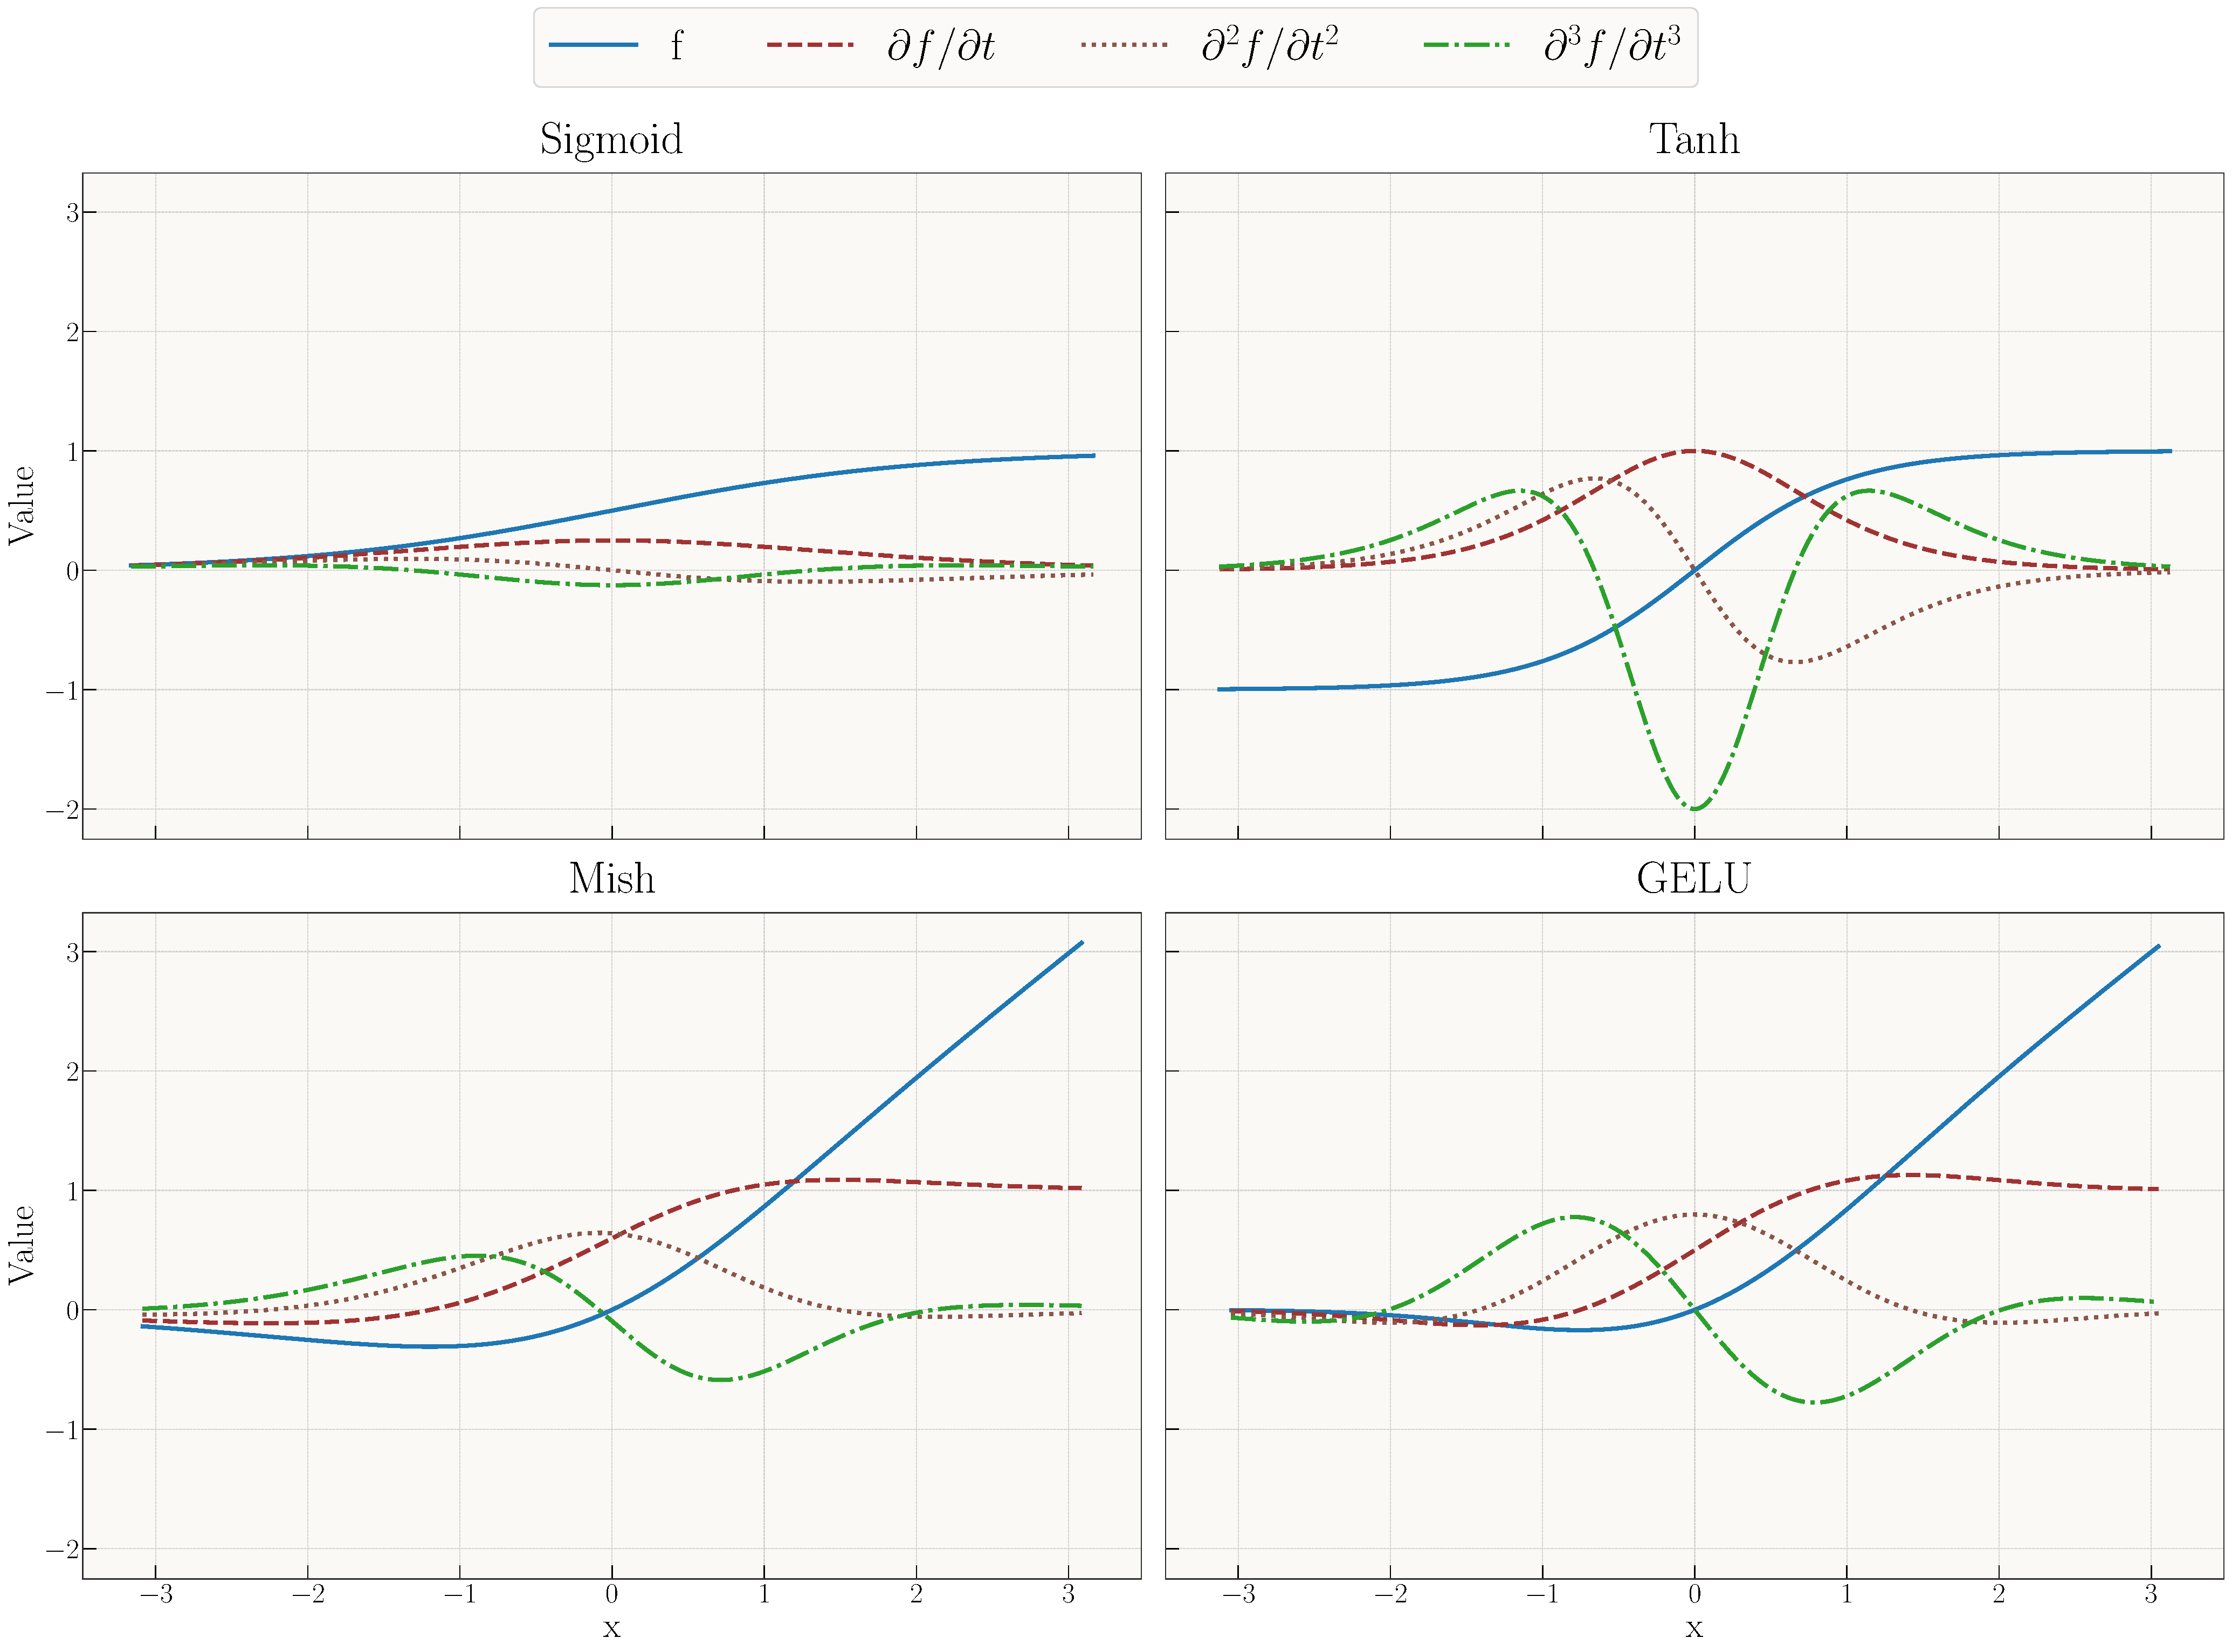
\includegraphics[width=0.8\textwidth]{all_activations_shared_legend.pdf}
  \caption[Activation functions and their first three derivatives]{Common activation functions and their first three derivatives. All of
  GELU, Mish, tanh and the logistic sigmoid are $C^\infty$, so the distinction is not
  smoothness but the \emph{reach} of the higher derivatives: for GELU and Mish the second
  and third derivatives are broad and decay slowly to zero, while for tanh and sigmoid they
  are sharply peaked near the origin and change sign, so curvature accumulates unevenly
  when such units are composed through depth. ReLU is shown for contrast; its second
  derivative is a distribution and it cannot be used in a Laplacian-based objective at all.}
  \label{fig:activation_derivatives}
\end{figure}

\paragraph{Initialisation.}
The standard schemes (Xavier/Glorot, scaling weight variance as $1/(n_{\rm in}+n_{\rm out})$, and Kaiming/He, scaling as $2/n_{\rm in}$ for rectified units) are designed to keep
forward activations and backward gradients from shrinking or exploding through
depth~\cite{GlorotBengio2010-Xavier,HeEtAl2015-KaimingInit}. That is necessary but not
sufficient when the loss contains second derivatives, because a scheme that stabilises
$\partial f/\partial x$ says nothing directly about $\partial^2 f/\partial x^2$. We use
Xavier-style initialisation with the smooth activations above, and---more consequentially
than any initialisation choice---zero-initialise the final layer of the backflow, so that
the ansatz begins exactly at the Slater nodes and the learned nodal deformation grows from
nothing rather than from noise (\S\ref{sec:bf-init}).

None of this makes the Laplacian well conditioned; it only stops the network from making
it worse. The conditioning itself comes from the coordinate scaling, the soft-core pair
features and the analytic cusp of Chapter~\ref{ch:trial_wavefunction}, and is analysed in
Appendices~\ref{app:laplacian} and~\ref{app:coulomb}.


\section{Architectures for many-body wavefunctions}
\label{sec:architectures}

The feed-forward network of the previous section maps a fixed-size input vector to an
output. A many-body wavefunction is not a generic function of such a vector: identical
particles impose a permutation symmetry, and correlation is intrinsically
\emph{relational}---what one particle should do depends on where the others are. A plain
multilayer perceptron acting on the concatenated coordinates
$(\mathbf x_1,\dots,\mathbf x_N)$ respects neither property; it would have to learn the
symmetry from data, and its parameter count would grow with $N$. This section introduces
the two architecture classes that build the required structure in, permutation-invariant pooling and message passing, and situates the specific message-passing network used in
this thesis as one instance of the latter.

\subsection{Permutation symmetry and equivariance}
For identical particles the modulus $|\Psi|$ is invariant under exchange (the sign is
carried by the antisymmetric Slater reference of Chapter~\ref{ch:trial_wavefunction}).
The two learnable objects of the ansatz therefore have distinct symmetry requirements.
A scalar \emph{correlator} $f$ must be permutation-\emph{invariant},
\[
  f(P_\sigma R)=f(R),
\]
while a per-particle \emph{backflow} displacement field $\mathbf g=(\mathbf g_1,\dots,\mathbf g_N)$
must be permutation-\emph{equivariant},
\[
  \mathbf g(P_\sigma R)=P_\sigma\,\mathbf g(R),
\]
for any permutation $\sigma$ (here $P_\sigma$ relabels the particles). Enforcing these by
construction is both more data-efficient than learning them and yields a parameter count
independent of $N$, because the same shared maps are applied to every particle and pair.

\subsection{Permutation-invariant pooling: DeepSets}
The simplest way to build an invariant function is to embed each particle independently
and pool the embeddings symmetrically. This is the DeepSets
construction~\cite{Zaheer2017-DeepSets}: any suitably regular permutation-invariant
function admits the form
\[
  f(R)=\rho\!\Big(\textstyle\sum_i \phi(\mathbf x_i)\Big),
\]
with a per-particle embedding $\phi$, a symmetric pool $\sum_i$, and a readout $\rho$. A
two-body extension encodes pairs, $\phi(\mathbf x_i,\mathbf x_j)$, and pools over them,
capturing pairwise correlation. What characterises this class is that each particle, or pair, is embedded \emph{independently} and only then pooled: no information is exchanged
between particles before the pool. We refer to such networks as \emph{separable}, and
they serve as the non-message-passing baseline for the correlator.

\subsection{Message passing and graph networks}
To let a particle's representation depend on the others' in an iterated, higher-order
way, one places the particles on a graph---nodes are particles, edges are
pairs---and passes learned messages along the edges~\cite{Gilmer2017-MPNN,Battaglia2018-GraphNetworks}.
In a generic round $\ell$, each edge gathers information from its endpoint nodes and each
node aggregates its incoming edge messages,
\[
  \mathbf m_{ij}^{(\ell)} = \phi_e\!\big(\mathbf h_i^{(\ell)},\mathbf h_j^{(\ell)},\mathbf e_{ij}^{(\ell)}\big),
  \qquad
  \mathbf h_i^{(\ell+1)} = \phi_v\!\Big(\mathbf h_i^{(\ell)},\ \textstyle\operatorname*{Agg}_{j\neq i}\mathbf m_{ij}^{(\ell)}\Big),
\]
with shared maps $\phi_e,\phi_v$ and a symmetric aggregation $\operatorname{Agg}$, so that
permutation equivariance holds by construction; a final readout produces an invariant
scalar (correlator) or an equivariant field (backflow). Both DeepSets and message passing
use pairwise information, but only message passing lets that information
\emph{propagate}: after several rounds a particle's representation reflects not just its
neighbours but their neighbours' responses. This iterated propagation is what we call the
\emph{relational channel}, and asking what it buys, in the correlator and in the backflow, is one of the central questions of this thesis. Message passing has been used
in exactly this spirit for neural quantum states of extended fermion
systems~\cite{Pescia2024-MessagePassingNQS,KimEtAl2023-UltracoldFermiNQS}.

\subsection{The CTNN: one message-passing instance}
\label{sec:ctnn-theory}
The message-passing correlator and backflow studied here are realised by a particular
network we refer to as the \emph{CTNN}: a copresheaf-style message-passing network that
maintains explicit \emph{node and edge} features and transports information between them
through learned maps, rather than recomputing and discarding one-shot messages. The
correlator iterates this exchange over a down/up ``V-cycle''; the backflow applies a
single such copresheaf round. Its concrete update equations, hidden dimensions, and
parameter counts are specified in the Methods chapter
(\S\ref{subsec:ctnn-backflow}, Eqs.~\eqref{eq:ctnn-edge}--\eqref{eq:ctnn-node}). Two things follow. First, the CTNN is \emph{one} concrete realisation of
the message-passing class defined above, and the comparison run in this thesis is between two
specific inductive biases---the CTNN against a DeepSets-type separable baseline---not between
the classes they belong to. Conclusions are stated for message passing \emph{as instantiated
by the CTNN, relative to the separable baseline studied here}; whether they generalise to
other message-passing neural quantum states is a plausible extrapolation and not something
these experiments test. Wherever we
contrast a ``message-passing'' network with a ``separable'' one, the separable member is
a DeepSets-type network and the message-passing member is the CTNN. Second, we write
``copresheaf-\emph{style}'' deliberately: the name reflects the node/edge transport
structure of the updates, not a claim to a formal sheaf-theoretic construction.

\subsection{Relevance to the ansatz}
Both learnable objects of the ansatz---the Jastrow correlator and the coordinate
backflow---can be built in either form: as a separable DeepSets-type network, or as the
message-passing CTNN. Holding everything else fixed and varying only this choice isolates
the effect of the relational channel, which Chapter~\ref{ch:kernel} analyses through the
geometry of the tangent kernel introduced in \S\ref{sec:theory-tangent-kernel}.

\section{Approximation theory and its limits}
\label{sec:nn_approximation}

The usual justification for using a neural network as a variational ansatz is that it can
represent anything. That argument needs disposing of early, since this thesis is about what
happens after it stops being relevant.

The universal approximation theorems say that a single hidden layer with a non-polynomial
activation is dense in $C(K)$ on compacta: for any continuous $f$ and any $\varepsilon>0$
there exist a width and a parameter vector achieving
$\sup_{x\in K}|f(x)-f_\theta(x)|<\varepsilon$~\cite{Cybenko1989,HORNIK1991251,LeshnoEtAl1993-NonpolyActivationUniversality}.
They establish one thing, best put negatively: there is no \emph{fundamental}
representability obstruction. They say nothing about the particular $20$k--$236$k networks
used here, nor about whether gradient-based training will find such a representation, at
what sample cost, or how the answer depends on the parameterisation. The existence proofs
are non-constructive, the widths they guarantee are astronomical, and the same function can
be represented by two networks whose optimisation behaviour is entirely different---which is,
in miniature, the comparison Chapter~\ref{ch:kernel} makes.

One further result does more than assert possibility. In high dimension a generic
continuous target requires a network size growing exponentially in $d$, so approximation
alone cannot explain why these methods work at all in $Nd$ dimensions.
The escapes are all statements about \emph{structure}, not capacity: targets of
finite Barron norm admit dimension-independent
rates~\cite{Barron1993-UniversalApprox}; compositional targets admit efficient
representation by deep networks when the composition matches the architecture; and imposing a symmetry removes the redundant
copies the network would otherwise have to learn, reducing the burden on the representation
rather than the dimension of the domain. The last of these is the one we exploit
directly, and the middle one is why the message-passing architectures of
\S\ref{sec:architectures} deserve attention: their usefulness comes from a compositional
form matching the relational structure of the physics, not from added capacity.

The rest of the thesis therefore assumes representability and measures the other things:
trainability, conditioning, and the geometry of the parameterisation.


\section{Residual objectives and their difficulties}
\label{sec:pinns}

In scientific applications the governing equations already encode most of what is known
about a system, and a model fitted only to data throws that information away.
\emph{Physics-informed neural networks} (PINNs)~\cite{raissi2019pinns} put it back by
penalising the residual of the equation itself: for a differential operator $\mathcal N$ and
a network $u_\theta$, the loss is a sampled sum of $|\mathcal N[u_\theta](\xi_j)|^2$ over
collocation points $\{\xi_j\}$, together with boundary and data terms. Training a network
against a differential operator predates the name by two
decades~\cite{Lagaris1998-ANNforODEPDE}; what \cite{raissi2019pinns} added was automatic
differentiation, which evaluates $\nabla u_\theta$ and $\Delta u_\theta$ exactly and cheaply
enough that the residual can drive the optimisation directly.

Four difficulties follow from differentiating through the operator, and each recurs by name
in the results of this thesis~\cite{De_Ryck_2024}.

\emph{Approximation in Sobolev norms.} Universal approximation controls function error in
$L^2$ or $L^\infty$, but a strong residual depends on \emph{derivatives}. Making it small
requires approximation in $W^{\ell,p}$ with $\ell$ the order of the equation, which forces
smooth activations for $\ell\ge2$ and architecture choices that control higher derivatives.
This is why the activation here is chosen for its second derivative, not its values.

\emph{Residual-to-error stability.} A small residual implies a small solution error only
where the forward problem is stable. This is why a small residual is never taken here as
evidence of a good state without an independent energy evaluation.

\emph{Sampling.} Collocation minimises a sampled surrogate of a continuum loss, and the
empirical residual can be small while the population residual is not. In this setting the
question becomes whether an importance-weighted estimator has a finite variance at all,
which is what bounds the Markov-chain-free programme of Chapter~\ref{ch:kernel}.

\emph{Conditioning.} Residual losses couple terms of disparate scale and produce
ill-conditioned gradient dynamics; in the linearised view, convergence is governed by the
spectrum of a problem-dependent kernel. That spectrum is the subject of the entire
tangent-kernel analysis.

The last of these determined the design of the collocation programme. A strong-form residual
that differentiates through the Laplacian meets a structural obstruction as soon as it is
asked to train a nodal surface, because the learning signal lives where $E_L$ diverges. The
weak form keeps the local energy as a detached reward and never differentiates it, and so
avoids the obstruction; Appendix~\ref{app:catch22} shows why, and it is the reason the
collocation programme takes the form it does.

\section{Constraints carried into the method}
\label{sec:ml_summary}

The two traditions of this chapter and the last have been describing the same objects in
different words. The quantum geometric tensor of variational Monte Carlo is the Fisher
metric of information geometry; stochastic reconfiguration is natural-gradient descent
under it; the neural tangent kernel is that metric's Gram dual; and the sampling measure a
physicist chooses for a Metropolis chain is what a statistician calls a proposal
distribution. Neither community needs the other's vocabulary in order to do its own work, which is why
the identifications are easy to miss. They matter here because the architecture determines
the spectrum of that metric, the optimiser inverts it, and the sampling measure determines
how well it can be estimated.

Four properties of this problem bear on that metric.

\emph{The objective contains a second-order operator.} The local energy carries a
Laplacian, so training differentiates through second derivatives of the network. This is
what dictates smooth activations, controlled initialisation, and a determinant that is
never asked to do anything violent (\S\ref{sec:ffnn}).

\emph{The interaction is singular, and the state carries nodes.} The Coulomb term diverges
at coalescence, and the trial function vanishes on a surface whose location is itself being
learned. Both are places where $E_L=\hat H\Psi/\Psi$ can blow up, and the cusp conditions
of \S\ref{subsec:cusp} say that the first divergence can be cancelled analytically if the
short-range form is built in, not learned.

\emph{The measure is part of the method.} The objective is an expectation under
$|\Psi_\theta|^2$, so the sampling distribution enters the gradient, the metric, and the
estimate of both. Whether that metric can be estimated at all turns out to decide whether
preconditioning helps or hurts (\S\ref{sec:theory-tangent-kernel}).

\emph{Correlation is relational.} What one electron should do depends on where the others
are, and the two architecture classes of \S\ref{sec:architectures} differ precisely in how
far that dependence is allowed to propagate.

The first two are met by construction in Chapter~\ref{ch:trial_wavefunction}, which
hard-wires antisymmetry and the cusp and conditions the geometry so that the learned part
can remain small and smooth. The third is treated in Chapter~\ref{ch:optimisation}, where
the sampling measure is a design variable rather than a fixed background. The fourth is not
settled here: both architectures are constructed, and the comparison between them is
reported in Chapter~\ref{ch:kernel}.

